\section{Testing and Results}
\subsection{Testing Procedure}
To validate the functionality and performance of the system, a structured testing procedure was employed. Each aspect of the system was rigorously examined to ensure reliability and accuracy under real-world conditions.

\subsubsection{System Initialization and Peripheral Verification}
\begin{enumerate}[leftmargin=2em]
    \item Power on the STM32F0 Discovery board and ensure stable voltage levels across all peripherals.
    \item Verify system clock configuration by outputting the clock frequency to the console and ensuring it matches the expected 48 MHz.
    \item Test GPIO pin configurations by probing each pin and confirming the expected input/output states using an oscilloscope.
    \item Check ADC and DAC initialization by generating a test analog signal using a function generator and confirming correct ADC readings and DAC voltage outputs using a multimeter.
    \item Initialize the OLED display and verify proper communication via SPI by displaying test data.
\end{enumerate}

\subsubsection{Frequency Measurement Validation}
\begin{enumerate}[leftmargin=2em]
    \item Generate a square-wave signal (max. 0–3.3 V amplitude) using a function generator at variable frequencies up to 80 MHz~\cite{uvic_equipment_handbook}.
    \item Connect the signal to PA2 and monitor the EXTI2 interrupt behavior using the debugger or console outputs.
    \item Measure the time elapsed between two rising edges of the input signal using TIM2 and confirm accuracy by comparing the calculated frequency to the function generator's set frequency.
    \item Determine the minimum detectable frequency by lowering the input signal frequency until the system fails to provide consistent measurements.
    \item Determine the maximum detectable frequency by increasing the input signal frequency until the timer fails to capture events accurately.
\end{enumerate}



\subsubsection{Resistance Calculation Validation}
\begin{enumerate}[leftmargin=2em]
    \item Connect a potentiometer to PA5 and adjust its resistance across the full range (0–5 k$\Omega$).
    \item Confirm ADC readings at various potentiometer positions by comparing the measured resistance (using the conversion from ADC to resistance) to values obtained using a multimeter.
    \item Validate real-time updates on the OLED display for resistance measurements using the console output or the OLED output.
\end{enumerate}

\subsubsection{Mode Switching Functionality}
\begin{enumerate}[leftmargin=2em]
    \item Test the system's response to pressing the USER button (PA0) by toggling between NE555 Timer Mode and Function Generator Mode.
    \item Ensure proper reconfiguration of EXTI interrupts for PA1 and PA2 when switching modes.
    \item Validate that frequency measurements from the correct input source are displayed on the OLED after each mode switch.
    \item Confirm seamless transitions without data loss or system crashes.
\end{enumerate}

\subsubsection{Signal Monitoring and DAC Control}
\begin{enumerate}[leftmargin=2em]
    \item Adjust the potentiometer and monitor the real-time ADC readings.
    \item Validate DAC outputs by connecting an oscilloscope to PA4 and confirming the output voltage corresponds to the scaled ADC input.
    \item Ensure that the DAC signal drives the optocoupler to adjust the PWM frequency and duty cycle of the NE555 timer circuit.
    \item Verify continuous synchronization between ADC input, DAC output, and OLED display updates.
\end{enumerate}

\subsubsection{Noise and Stability Testing}
\begin{enumerate}[leftmargin=2em]
    \item Introduce electrical noise to the system using a signal generator or by varying the power supply voltage.
    \item Verify the robustness of the ADC readings and DAC outputs under noisy conditions by observing the stability of displayed data and oscilloscope waveforms.
    \item Test the impact of simultaneous mode switching and signal input variations on system performance.
    \item Confirm the effectiveness of decoupling capacitors in mitigating noise.
\end{enumerate}

\subsection{Results}
The system demonstrated robust performance across all testing scenarios, meeting or exceeding the project requirements.

\subsubsection{Frequency Measurement Performance}\label{sec:freq_measurement}
In the STM32 microcontroller, the ARR in the timer is limited 32 bits. Therefore, the maximum count is determined by the following:

$$N_{\text{max}} = 2^{32} - 1 = 4,294,967,295$$

Therefore, the \textbf{minimum frequency} would be:
$$f_{\text{min}} = \frac{f_{\text{clock}}}{N_{\text{max}}} = \frac{48,000,000}{4,294,967,295} \approx 0.0112 \text{ Hz}$$

\noindent Moreover, the graph in Figure \ref{fig:fmeasured_graph} shows the plot of measured frequencies with the frequencies from the function generator. And the second graph (Figure \ref{fig:error_graph}) shows the percentage error from the measured frequencies against the expected frequencies.

\begin{figure}[H]
    \centering
    \begin{tikzpicture}
    \begin{axis}[
        xlabel={Frequency (Hz)},       % Label for the x-axis
        ylabel={Measured Frequency (Hz)},       % Label for the y-axis
        grid=both,               % Add a grid
    grid style={dotted},
        width=12cm,              % Adjust width
        height=8cm,              % Adjust height
        legend style={at={(0.5,-0.2)}, anchor=north, legend columns=-1},
        legend entries={Expected Curve, Actual Curve},
        legend cell align={left}
    ]
        \addplot[
            color=blue,         % Line color,
            dashed,
            mark=*              % Marker style
        ] 
        table[
            col sep=comma,      % Column separator (comma for CSV files)
            x=Input,                % Specify column for x
            y=Expected                 % Specify column for y
        ] {tables/freq_measurements.csv};

        \addplot[
            color=red,         % Line color,
            mark=*              % Marker style
        ] 
        table[
            col sep=comma,      % Column separator (comma for CSV files)
            x=Input,                % Specify column for x
            y=Measured                 % Specify column for y
        ] {tables/freq_measurements.csv};
   
    \end{axis}
\end{tikzpicture}
    \caption{Graph of Function Generatior Frequency vs. Measured Frequency from the MCU}
    \label{fig:fmeasured_graph}
\end{figure}

\begin{figure}[H]
    \centering
    \begin{tikzpicture}
    \begin{axis}[
        xlabel={Frequency (Hz)},       % Label for the x-axis
        ylabel={Percentage Error (\%)},       % Label for the y-axis
        grid=both,               % Add a grid
    grid style={dotted},
        width=12cm,              % Adjust width
        height=8cm,              % Adjust height
        legend style={at={(0.5,-0.2)}, anchor=north, legend columns=-1},
        legend cell align={left}
    ]

        \addplot[
            color=cyan,         % Line color,
            mark=*              % Marker style
        ] 
        table[
            col sep=comma,      % Column separator (comma for CSV files)
            x=Input,                % Specify column for x
            y=Error                 % Specify column for y
        ] {tables/freq_measurements.csv};
   
    \end{axis}
\end{tikzpicture}
    \caption{Graph of Percentage Error against Inputted Frequency}
    \label{fig:error_graph}
\end{figure}

Judging by the graphs above, the system can only read up to 480 kHz, with an error of less than 9\%. Therefore, the maximum frequency is \textbf{480 kHz}.

Higher frequencies have smaller time period, $T$. The system clock counts the number of counts ($N$) using the TIM2 counter between two rising edges using the prescaler value set at zero (i.e. at system clock frequency of 48 MHz).  However, the system clock lacks adequate sampling frequency to measure very small periods, which makes the frequency measurement inaccurate.

For a 48 MHz clock, each clock cycle is \textbf{20.83 ns}. The number of counts, \( N \), recorded by the timer for one signal period ($T$) is:

\begin{equation}\label{number_of_counts}
    N = T \times f_{\text{clock}}
\end{equation}

Where $T$ is the period of the signal (in seconds), and $f_{\text{clock}}$ is the system clock frequency (48 MHz).

For example, a high-frequency signal like 600 kHz, the period, $T$ of the signal is:
$$T = \frac{1}{f_{\text{signal}}} = \frac{1}{600,000} = 1.6667 \, \mu\text{s}$$

Therefore, the number of counts for this frequency are:
$$N = T \times f_{\text{clock}} = 1.6667 \times 10^{-6} \times 48 \times 10^6 = 80 \, \text{counts}$$

With only 80 counts, only one missed or extra clock cycle introduces significant error. For example, a missing \textbf{1 clock cycle} changes $N$ to 79, resulting in:
    \[
    \text{Frequency error} = \frac{f_{\text{clock}}}{N} - \frac{f_{\text{clock}}}{N-1}
    \]
    \[
    \text{Error} = \frac{48,000,000}{80} - \frac{48,000,000}{79} \approx 600,000 - 607,595 = 7,595 \, \text{Hz}
    \]
This results in a \textbf{quantization error} of approximately \textbf{1.27\%} just from missing 1 clock cycle. However, it missed many clock cycles which gave a relative error of about 49.36\%. It is very likely caused by the following criteria:

\begin{itemize}[leftmargin=2em]
    \item  \textbf{Interrupt Latency:} The microcontroller might not be able to process interrupts fast enough due to delays in handling and returning from interrupts. Therefore, the interrupt handling has caused some synchronization issues.
    \item \textbf{Jitter and Noise:} At such high frequencies, any signal noise or jitter can cause additional rising edges to be detected erroneously or edges to be missed altogether, introducing further inaccuracies.
\end{itemize}

\noindent To summarize, the system suceeded with the following results:

\begin{itemize}[leftmargin=2em]
    \item \textbf{Accuracy:} Measured frequencies with a relative error within 9\% from the function generator's reference values across a range of \textbf{0.0112 Hz to 480 kHz}.
    \item \textbf{Minimum Detectable Frequency:} \textbf{0.0112 Hz}, limited by the timer's ability to measure long periods without overflow.
    \item \textbf{Maximum Detectable Frequency:} \textbf{480 kHz}, constrained by EXTI interrupt latency and TIM2 resolution.
\end{itemize}

\subsubsection{Resistance Measurement Performance}
\begin{itemize}[leftmargin=2em]
    \item \textbf{Accuracy:} Resistance calculations matched multimeter readings within 5\% across the full range of the potentiometer (0–5 k$\Omega$).
    \item \textbf{Response Time:} Real-time updates to the OLED display occurred with minimal latency, ensuring user-friendly interaction.
\end{itemize}

\subsubsection{NE555 Timer Frequencies against Potentiometer Readings}

The graph in Figure \ref{fig:ne555_graph} below shows the NE555 timer frequency readings with varying potentiometer resistance. (The blue curve shows the frequencies measured from the MCU, and the red curve shows the actual frequency measured from the oscilloscope.)

% NE555 Timer Graph
\begin{figure}[H]
    \centering
    % Begin the figure environment
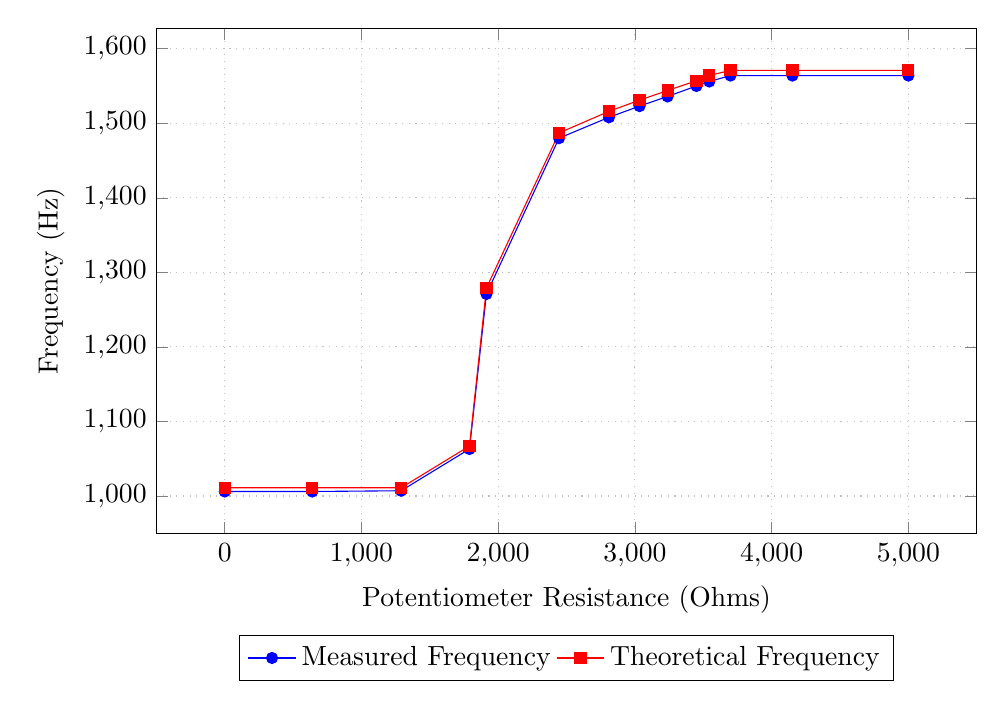
\begin{tikzpicture}

    % Define the table and plot layout
    \begin{axis}[
        width=12cm,
        height=8cm,
        grid=both,
        grid style={dotted},
        xlabel={Potentiometer Resistance (Ohms)},
        ylabel={Frequency (Hz)},
        legend style={at={(0.5,-0.2)}, anchor=north, legend columns=-1},
        legend entries={Measured Frequency, Theoretical Frequency},
        legend cell align={left}
    ]
    
    % Measured Frequency Plot
    \addplot[color=blue, mark=*] table {
    0    1006
    640  1006
    1290 1007
    1790 1063
    1914 1271
    2445 1480
    2810 1508
    3034 1523
    3239 1536
    3450 1550
    3544 1556
    3699 1564
    4152 1564
    5000 1564
    };
    
    % Theoretical Frequency Plot
    \addplot[color=red, mark=square*] table {
    0    1011
    640  1011
    1290 1011
    1790 1067
    1914 1279
    2445 1487
    2810 1516
    3034 1531
    3239 1544
    3450 1557
    3544 1564
    3699 1571
    4152 1571
    5000 1571
    };
    
    \end{axis}
\end{tikzpicture}
    \caption{Graph of 555 Timer Frequency against Potentiometer Resistance}
    \label{fig:ne555_graph}
\end{figure}

It is observed that the frequency remains constant at 1011 Hz until 1290 $\Omega$. After 1290 $\Omega$, the frequency skyrockets until at 3700 $\Omega$, it gradually reaches a constant value at 1571 Hz. Therefore, with the DAC voltages generating from 0.126-2.23 V, the system can generate PWM signals through the NE555 timer at frequencies ranging from \textbf{1011 Hz} to \textbf{1571 Hz}.

\subsubsection{Mode Switching Reliability}
\begin{itemize}[leftmargin=2em]
    \item \textbf{Seamless Transitions:} Mode switches occurred instantaneously, with accurate updates to frequency and resistance measurements.
    \item \textbf{Interrupt Handling:} No missed events or system crashes were observed during rapid mode toggling.
\end{itemize}

\subsubsection{Noise Mitigation and Stability}
\begin{itemize}[leftmargin=2em]
    \item \textbf{Noise Rejection:} Effective decoupling capacitors \cite{ne555-timer-datasheet} and robust interrupt-driven control minimized noise-induced errors.
    \item \textbf{Stable Operation:} The system maintained consistent performance even under noisy conditions and power supply variations.
\end{itemize}

\subsubsection{System Limitations}
\begin{itemize}[leftmargin=2em]
    \item The maximum detectable frequency (480 kHz) is limited by EXTI and TIM2 latency, and further optimization may require higher-performance hardware.
    \item The ADC sampling rate (239.5 clock cycles) \cite{interfacex} restricts the system's ability to process rapidly changing analog inputs.
\end{itemize}
